\chapter{Anhang}

\begin{figure}[htb]
  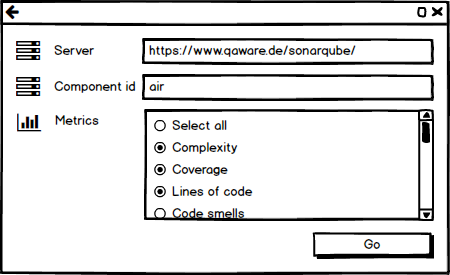
\includegraphics[width=.8\textwidth]{figures/sonarqube-import}
  \caption{Low-Fi Prototyp für den Import eines neuen Projekts anhand des Beispiels SonarQube}
  \label{fig:sonarqube-import}
\end{figure}

\begin{figure}[htb]
  \centering
  \begin{subfigure}[b]{\fwidth}
    \centering
    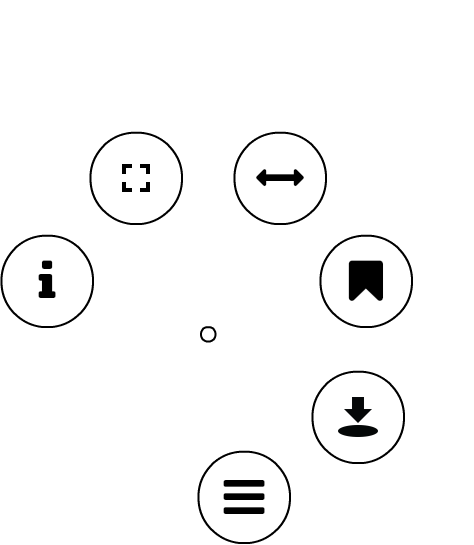
\includegraphics[scale=0.45]{figures/edge-contextmenu}
    \subcaption{Initialer Zustand} \label{fig:edge-contextmenu-initial}
  \end{subfigure}
  \hfill
  \begin{subfigure}[b]{\fwidth}
    \centering
    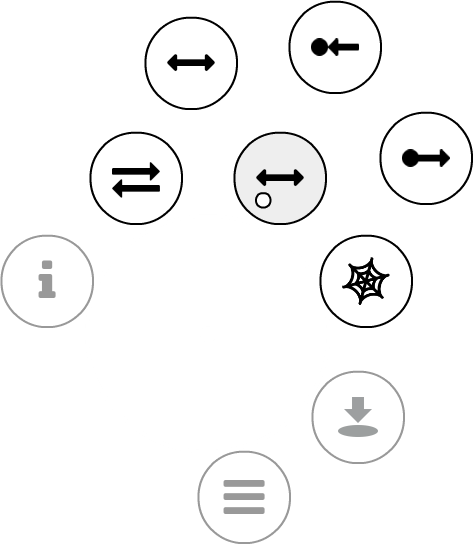
\includegraphics[scale=0.45]{figures/edge-contextmenu-connections}
    \subcaption{Unterauswahl für Verbindungen} \label{fig:edge-contextmenu-connections}
  \end{subfigure}
  \caption{Kontextmenü für einen inneren Knoten} \label{fig:edge-contextmenu}
\end{figure}

\begin{figure}[htb]
  \centering
  \begin{subfigure}[b]{\fwidth}
    \centering
    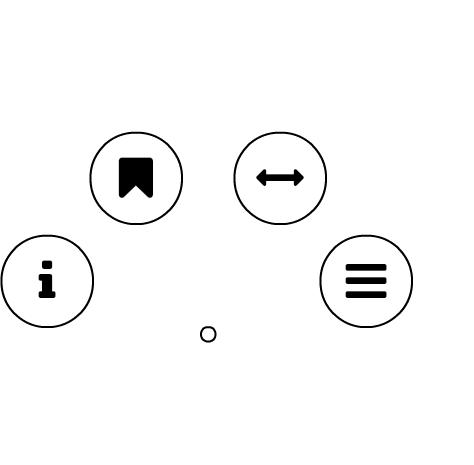
\includegraphics[scale=0.45]{figures/root-contextmenu}
    \subcaption{Initialer Zustand} \label{fig:root-contextmenu-initial}
  \end{subfigure}
  \hfill
  \begin{subfigure}[b]{\fwidth}
    \centering
    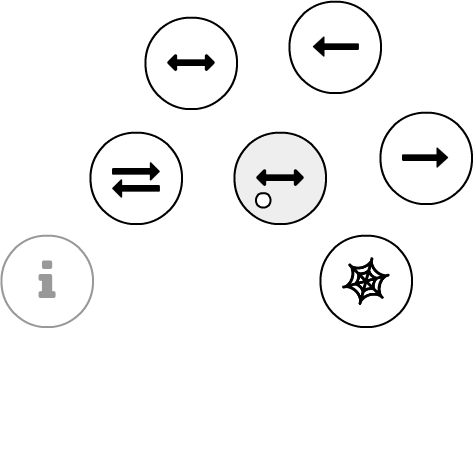
\includegraphics[scale=0.45]{figures/root-contextmenu-connections}
    \subcaption{Unterauswahl für Verbindungen} \label{fig:root-contextmenu-connections}
  \end{subfigure}
  \caption{Kontextmenü für eine Wurzel} \label{fig:root-contextmenu}
\end{figure}